\section{Mathematical formulation}
\label{chap2:sec:mathematical_formulation}

The steady-state convection-diffusion problem is addressed in two dimensions and formulated with the Cartesian coordinate system considering $\bm{x}\coloneqq\left(x,y\right)$.
Let $\Omega$ be an open bounded domain of $\mathbb{R}^{2}$ with boundary $\Gamma$, partitioned into three non-overlapping and possibly empty subsets, $\Gamma^{\textrm{D}}$, $\Gamma^{\textrm{N}}$, and $\Gamma^{\textrm{R}}$, such that $\Gamma=\Gamma^{\textrm{D}}\cup\Gamma^{\textrm{N}}\cup\Gamma^{\textrm{R}}$.
The boundary and the interface are regular Jordan curves, that is, simple and closed curves, and admit a known local parameterization.
Vector $\bm{n}=\left(n_{x},n_{y}\right)\coloneqq\left(n_{x}\left(\bm{x}\right),n_{y}\left(\bm{x}\right)\right)$ stands for the outward unit normal vector to $\Gamma$ at point $\bm{x}$ on the boundary (see Figure~\ref{chap2:fig:mathematical_formulation_domain}).

\begin{figure}[!htb]
\centering
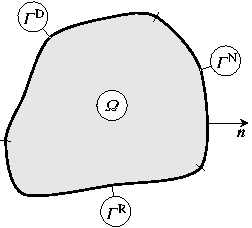
\includegraphics[width=4.5cm]{chap2/include/tikz/curved_domain}
\caption{Example of arbitrary curved domain with boundary subsets and outward unit normal vector.}
\label{chap2:fig:mathematical_formulation_domain}
\end{figure}

\subsection{Convection-diffusion model}
\label{chap2:subsec:mathematical_formulation_convection_diffusion_model}

The governing equation for temperature function $\phi\coloneqq\phi\left(\bm{x}\right)$ is given as
\begin{equation}
\nabla\cdot\left(\bm{u}\phi-\kappa\nabla\phi\right)=f,\quad\text{ in }\Omega,
\label{chap2:eq:mathematical_formulation_convdiff}
\end{equation}
where $\bm{u}\coloneqq\left(u_{x},u_{y}\right)\coloneqq\left(u_{x}\left(\bm{x}\right),u_{y}\left(\bm{x}\right)\right)$ is the velocity vector function multiplied by the heat capacity and density of the associated material, $\kappa\coloneqq\kappa\left(\bm{x}\right)$ is the thermal conductivity function, and $f\coloneqq f\left(\bm{x}\right)$ is the heat source function (a negative value implies a heat sink).
All functions are assumed to be regular and bounded in the domain.
To complete Equation~\cref{chap2:eq:mathematical_formulation_convdiff}, boundary subsets $\Gamma^{\textrm{D}}$, $\Gamma^{\textrm{N}}$, and $\Gamma^{\textrm{R}}$ are prescribed with the following boundary conditions:
\begin{itemize}
\item On boundary subset $\Gamma^{\textrm{D}}$, a Dirichlet boundary condition is prescribed, given as
\begin{equation}
\label{chap2:eq:mathematical_formulation_dirichlet}
\phi=g^{\textrm{D}},\quad\text{on }\Gamma^{\textrm{D}},
\end{equation}
where $g^{\textrm{D}}\coloneqq g^{\textrm{D}}\left(\bm{x}\right)$ is a given regular function.
\item On boundary subset $\Gamma^{\textrm{N}}$, a Neumann boundary condition is prescribed, given as
\begin{equation}
\label{chap2:eq:mathematical_formulation_neumann}
-\kappa\nabla\phi\cdot\bm{n}=g^{\textrm{N}},\quad\text{on }\Gamma^{\textrm{N}},
\end{equation}
where $g^{\textrm{N}}\coloneqq g^{\textrm{N}}\left(\bm{x}\right)$ is a given regular function.
\item On boundary subset $\Gamma^{\textrm{R}}$, a Robin boundary condition is prescribed, given as
\begin{equation}
\label{chap2:eq:mathematical_formulation_robin}
\alpha^{\textrm{R}}\phi+\beta^{\textrm{R}}\nabla\phi\cdot\bm{n}=g^{\textrm{R}},\quad\text{on }\Gamma^{\textrm{R}},
\end{equation}
where $g^{\textrm{R}}\coloneqq g^{\textrm{R}}\left(\bm{x}\right)$, $\alpha^{\textrm{R}}\coloneqq\alpha^{\textrm{R}}\left(\bm{x}\right)$, and $\beta^{\textrm{R}}\coloneqq\beta^{\textrm{R}}\left(\bm{x}\right)$ are given regular functions.
For instance, if $\alpha^{\textrm{R}}\left(\bm{x}\right)\coloneqq\bm{u}\left(\bm{x}\right)\cdot\bm{n}\left(\bm{x}\right)$ and $\beta^{\textrm{R}}\left(\bm{x}\right)\coloneqq-\kappa\left(\bm{x}\right)$, then the Robin boundary condition represents a total heat flux boundary condition.
The Robin boundary condition can also be used to prescribe mixed boundary conditions of Dirichlet and Neumann types.
\end{itemize}

\subsection{Polygonal meshes}
\label{chap2:subsec:mathematical_formulation_polygonal_meshes}

A general polygonal mesh denoted as $\mathcal{M}$ discretizes the subdomain $\Omega$ and consists of $n$ non-overlapping convex polygonal cells (triangles, quadrangles, etc.).
Cells are denoted as $c_{i}$ with $i\in\mathcal{I}=\lbrace 1,\ldots,n\rbrace$.
Inner edges are denoted as $e_{ij}$ with $j\neq i$ and $i,j\in\mathcal{I}$ and correspond to the edges shared between neighbour cells $c_{i}$ and $c_{j}$ and, therefore, $e_{ij}=c_{i}\cap c_{j}$.
Boundary edges are denoted as $e_{iF}$ with $i\in\mathcal{I}^{F}$, $F\in\lbrace\textrm{D},\textrm{N},\textrm{R}\rbrace$, and correspond to the edges of cells $c_{i}$ approximating boundary subsets $\Gamma^{F}$ (for the sake of simplicity, each cell has at most one boundary edge).
Subset $\mathcal{I}^{F}\subset\mathcal{I}$ gathers the indices and $n^{F}$ is the number of the cells with a boundary edge approximating boundary subset $\Gamma^{F}$.
The vertices of the boundary edges fall on the curves of the associated boundary subsets.

Table~\ref{chap2:tab:mathematical_formulation_notations} introduces the geometric properties for the cells and edges and Figures~\ref{chap2:fig:mathematical_formulation_notations} provides a schematic representation.
Notice that inner edge $e_{ij}$ is also denoted as $e_{ji}$ and, therefore, reference and quadrature points are the same, that is, $\bm{m}_{ij}=\bm{m}_{ji}$ and $\bm{q}_{ij,r}=\bm{q}_{ji,r}$, whereas outward unit normal vectors are antisymmetric, that is, $\bm{s}_{ij}=-\bm{s}_{ji}$.

\begin{table}[!htb]
\centering
\caption{Notation and geometric properties for the cells and edges.}
\label{chap2:tab:mathematical_formulation_notations}
\resizeboxlarger{
\begin{tabular}{@{}lllll@{}}
\toprule
Mesh elements & Notation & Properties & Definition & Choice\\
\midrule
\multirow{5}{*}{Cells} & \multirow{5}{*}{$c_{i}$} & $\partial c_{i}$ & Boundary & \\
& & $\vert c_{i}\vert$ & Area & \\
& & $\bm{m}_{i}=\left(m_{i,x},m_{i,y}\right)$ & Reference point (can be any point in $c_{i}$) & Centroid \\
& & $\bm{q}_{i,q}=\left(q_{i,q,x},q_{i,q,y}\right)$ & Quadrature points, $q=1,\ldots,Q$ & Gaussian \\
& & $\mathcal{N}_{i}$ & Indices of the adjacent cells and boundary subset & \\
\midrule
\multirow{4}{*}{Inner edges} & \multirow{4}{*}{$e_{ij}$} & $\vert e_{ij}\vert$ & Length & \\
& & $\bm{m}_{ij}=\left(m_{ij,x},m_{ij,y}\right)$ & Reference point (can be any point on $e_{ij}$) & Midpoint\\
& & $\bm{q}_{ij,r}=\left(q_{ij,r,x},q_{ij,r,y}\right)$ & Quadrature points, $r=1,\ldots,R$ & Gaussian \\
& & $\bm{s}_{ij}=\left(s_{ij,x},s_{ij,y}\right)$ & Outward unit normal vector from cell $c_{i}$ to cell $c_{j}$ & \\
\midrule
\multirow{4}{*}{Boundary edges} & \multirow{4}{*}{$e_{iF}$} & $\vert e_{iF}\vert$ & Length & \\
& & $\bm{m}_{iF}=\left(m_{iF,x},m_{iF,y}\right)$ & Reference point (can be any point on $e_{iF}$) & Midpoint\\
& & $\bm{q}_{iF,r}=\left(q_{iF,r,x},q_{iF,r,y}\right)$ & Quadrature points, $r=1,\ldots,R$ & Gaussian \\
& & $\bm{s}_{iF}=\left(s_{iF,x},s_{iF,y}\right)$ & Outward unit normal vector from $c_{i}$ & \\
\bottomrule
\end{tabular}
}
\end{table}
\vspace{1.0cm}

\begin{figure}[!htb]
\centering
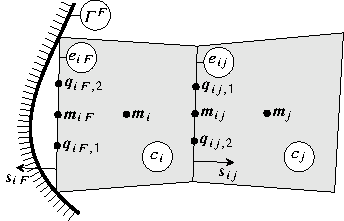
\includegraphics[height=4.5cm]{chap2/include/tikz/mesh2d_boundary}
\caption{Notation and geometric properties for the cells and edges.}
\label{chap2:fig:mathematical_formulation_notations}
\end{figure}

In the scope of work, keywords physical and computational distinguish the real domain from the discretized domain, respectively, and in this way, the following definitions are introduced:
\begin{itemize}
\item The computational domain, denoted as $\Omega_{\Delta}$, gathers all the cells and stands for a representative approximation of physical domain $\Omega$, given as
\begin{equation}
\Omega_{\Delta}=\bigcup_{i\in\mathcal{I}}c_{i}.
\end{equation}

\item The computational boundary, denoted as $\Gamma_{\Delta}$, gathers all the boundary edges and stands for a representative approximation of physical boundary $\Gamma$, given as
\begin{equation}
\Gamma_{\Delta}=\bigcup_{i\in\mathcal{I}^{F},F\in\lbrace\textrm{D},\textrm{N},\textrm{R}\rbrace}e_{iF}.
\end{equation}

\item The computational boundary subset, denoted as $\Gamma^{F}_{\Delta}$, $F\in\lbrace\textrm{D},\textrm{N},\textrm{R}\rbrace$, gathers all the boundary edges associated to a boundary subset and stands for a representative approximation of physical boundary subset $\Gamma^{F}$, given as
\begin{equation}
\Gamma^{F}_{\Delta}=\bigcup_{i\in\mathcal{I}^{F}}e_{iF}.
\end{equation}

\end{itemize}

\begin{myremark}
The curved physical domain, $\Omega$, and corresponding polygonal approximation, $\Omega_{\Delta}$, do not fully overlap as only polygonal meshes are considered.
For fine enough meshes, a mismatch of order $\mathcal{O}\left(h^{2}\right)$ is then expected between the physical and the computational boundaries, where $h$ is the characteristic mesh size.
Such mismatch represents a potential accuracy deterioration for any more than second-order accurate scheme.
\end{myremark}

% \begin{table}[!htb]
% \centering
% \caption{Mesh notations for the edges and cells.}
% \label{chap2:tab:mathematical_formulation_notations}
% \resizebox{\columnwidth}{!}{
% \begin{tabular}{@{}p{3.5cm}|p{3.5cm}|p{8.0cm}@{}}
% Mesh element & Notation & Definition\\
% \toprule
% \multirow{9}{*}{\begin{tabular}{@{}p{4.0cm}@{}}Cells\\$c_{i}$, $i\in\mathcal{I}$\end{tabular}} & $\partial c_{i}$ & -- Boundary\\
% & $\vert c_{i}\vert$ & -- Area\\
% & $\bm{m}_{i}=\left(m_{i,x},m_{i,y}\right)$ & -- Reference point, can be any point in $c_{i}$ \left(the centroid is used in this work\right)\\
% & $\bm{q}_{i,r}=\left(q_{i,r,x},q_{i,r,y}\right)$ & -- Quadrature points with $j=1,\ldots,R$ \left(Gaussian quadrature is used in this work\right)\\
% & $\mathcal{N}_{i}$ & -- Index set of the neighbor cells or boundary \left(von Neumann type neighborhood\right), $\mathcal{N}_{i}\subset\mathcal{I}\cup\lbrace\textrm{D},\textrm{N},\textrm{R}\rbrace$, such that index $k\in\mathcal{I}\cup\lbrace\textrm{D},\textrm{N},\textrm{R}\rbrace$ belongs to $\mathcal{N}_{i}$ if $e_{ik}$ is an edge of $c_{i}$\\
% \midrule
% \multirow{7}{*}{\begin{tabular}{@{}p{4.0cm}@{}}Inner edges\\$e_{ij}$, $i\in\mathcal{I}$, $j\in\mathcal{N}_{i}$\end{tabular}} & $\vert e_{ij}\vert$ & -- Length\\
% & $\bm{s}_{ij}=\left(n_{ij,x},n_{ij,y}\right)$ & -- Outward unit normal vector from cell $c_{i}$ to cell $c_{j}$ \left(notice that $\bm{s}_{ij}=-\bm{s}_{ji}$\right)\\
% & $\bm{m}_{ij}=\left(m_{ij,x},m_{ij,y}\right)$ & -- Reference point, can be any point in $e_{ij}$ \left(the midpoint is used in this work and notice that $\bm{m}_{ij}=\bm{m}_{ji}$\right)\\
% & $\bm{q}_{ij,r}=\left(q_{ij,r,x},q_{ij,r,y}\right)$ & -- Quadrature points with $r=1,\ldots,R$ \left(Gaussian quadrature is used in this work and notice that $\bm{q}_{ij,r}=\bm{q}_{ji,r}$\right)\\
% \midrule
% \multirow{7}{*}{\begin{tabular}{@{}p{4.0cm}@{}}Boundary edges\\$e_{iF}$, $i\in\mathcal{B_{M,F}}$, $F\in\lbrace\textrm{D},\textrm{N},\textrm{R}\rbrace$\end{tabular}} & $\vert e_{iF}\vert$ & -- Length\\
% & $\bm{s}_{iF}=\left(n_{iF,x},n_{iF,y}\right)$ & -- Outward unit normal vector from cell $c_{i}$ to the outside of the domain\\
% & $\bm{m}_{iF}=\left(m_{iF,x},m_{iF,y}\right)$ & -- Reference point, can be any point in $e_{iF}$ \left(the midpoint is used in this work\right)\\
% & $\bm{q}_{iF,r}=\left(q_{iF,r,x},q_{iF,r,y}\right)$ & -- Quadrature points with $r=1,\ldots,R$ \left(Gaussian quadrature is used in this work\right)\\
% \bottomrule
% \end{tabular}
% }
% \end{table}

%\begin{itemize}
%\item for any cell $c_{i}$, $\partial c_{i}$ denotes its boundary with area $\vert c_{i}\vert$.
%the reference cell point is denoted as $\bm{m}_{i}=\left(m_{i,x},m_{i,y}\right)$ which can be any point in $c_{i}$ \left(the centroid is considered in the present work\right).
%\item edge $e_{ij}$ with length $\vert e_{ij}\vert$ and $\bm{s}_{ij}=\left(n_{ij,x},n_{ij,y}\right)$ is the outward unit normal vector to $e_{ij}$ from $c_{i}$ to $c_{j}$, that is $\bm{s}_{ij}=-\bm{s}_{ji}$.
%the reference edge point is $m_{ij}=\left(m_{ij,x},m_{ij,y}\right)$ which can be any point on the edge $e_{ij}$ \left(the midpoint is considered in the present work\right).
%%\item if an edge of cell $c_{i}$ belongs to the boundary, the notation $e_{iF}$ is used, which turns more specific when necessary by setting $e_{iF}=e_{i\textrm{D}}$, $e_{i\textrm{N}}$, $e_{i\textrm{R}}$ when the edge belongs to $\Gamma_{\Delta,\textrm{D}}$, $\Gamma_{\Delta,\textrm{N}}$, or $\Gamma_{\Delta,\textrm{R}}$, respectively.
%\item for any edge $e_{ij}$, points $q_{ij,r}$, $r=1,\ldots,R$, denote the quadrature points and $\zeta_{r}$ the associated weights.
%\item for any cell $c_{i}$, the index set $\nu\left(i\right)\subset\lbrace\mathcal{C_M}\cup\{\textrm{D},\textrm{N},\textrm{R}\}\rbrace$ lists the neighbor cells or boundary, such that $j\in\nu\left(i\right)$ if $e_{ij}$ is a common edge between cells $c_{i}$ and $c_{j}$ or with the boundary $\Gamma_{\Delta,\textrm{D}}$, $\Gamma_{\Delta,\textrm{N}}$, or $\Gamma_{\Delta,\textrm{R}}$ if $j=\textrm{D},\textrm{N},\textrm{R}$, respectively.
%\end{itemize}

% end of file
